%(BEGIN_QUESTION)
% Copyright 2006, Tony R. Kuphaldt, released under the Creative Commons Attribution License (v 1.0)
% This means you may do almost anything with this work of mine, so long as you give me proper credit

I denne kretsen brukes en termistor for å styre effekt til en lampe:

$$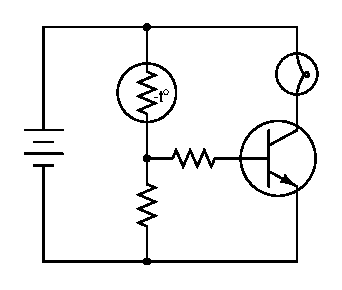
\includegraphics[width=15.5cm]{i00417x01.eps}$$

Når temperaturen øker, blir lampen sterkere eller svakere? Forklar svaret.

\underbar{file i00417}
%(END_QUESTION)





%(BEGIN_ANSWER)

Når temperaturen øker, synker resistansen til termistoren fordi den har negativ <alpha> (merk -t$^{o}$-symbolet inne i termistorboblen). Lavere termistorresistans betyr at spenningen på transistorens base (i forhold til emitter) blir mer positiv. Dette foroverpolariserer base-emitter PN-overgangen og slår på NPN-transistoren. Når transistoren leder mer, får lampen mer strøm og lyser sterkere.

%(END_ANSWER)





%(BEGIN_NOTES)

\vskip 20pt \vbox{\hrule \hbox{\strut \vrule{} {\bf Virtuell feilsøking} \vrule} \hrule}

Dette spørsmålet egner seg godt som en «virtuell feilsøking»-øvelse. Når du presenterer kretsdiagrammet for studentene, ser du først for deg en bestemt feil i systemet. Deretter presenterer du ett eller flere symptomer på denne feilen (noe en operatør eller annen bruker kan observere). Studentene foreslår så ulike diagnostiske tester for å identifisere feiltype og feilsted, som om de var teknikere som feilsøkte systemet. Din oppgave er å fortelle hva resultatet ville blitt for hver foreslåtte test, og dokumentere resultatene slik at alle studentene kan se dem.

Under og etter øvelsen er det nyttig å stille oppfølgingsspørsmål som:

\begin{itemize}
\item{} Hva forteller resultatet av den siste diagnostiske testen om feilen?
\item{} Anta at resultatet av den siste testen hadde vært annerledes. Hva ville det i så fall fortalt om feilen?
\item{} Er den siste diagnostiske testen den beste vi kunne gjort?
\item{} Hva ville vært den ideelle testrekkefølgen for å finne feilen i færrest mulig trinn?
\end{itemize}


%INDEX% Measurement, temperature: thermistor

%(END_NOTES)
